%!TEX root = ../main.tex

\section{Architecture}
The system consists of a Microblaze processor, a DDR2 SDRAM memory, peripheral systems for Ethernet and UART interfacing, as well as units for cryptographic algorithms. All subsystems are connected to the processor via a PLB (Processor Local Bus) bus. Additional peripherals required during design include an interrupt controller and a timer. The interrupt controller manages interrupts from coming from the Ethernet, UART, and the timer. The timer is required by lwIP for time measurements. The architecture of the system is depicted in Figure \ref{fig:figure_5.1}.

% fig 5.1
\begin{figure}[H]
\centering
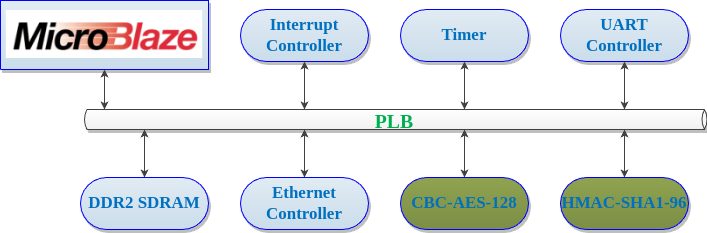
\includegraphics[width= 0.8\textwidth]{figure_5.1}\\
\caption{ High-level system architecture }
\label{fig:figure_5.1}
\end{figure}

Each peripheral system is assigned its own address range when integrated with Microblaze (Address Mapped IO). The transfer of data to and from the memory of the cryptographic peripheral systems is handled by Microblaze (i.e., there is no Direct Memory Access - DMA system). This is because the system does not operate in multipacket mode which means that it is not capable of processing more than one packet simultaneously. This is because lwIP does not utilize threading when deployed in bare-metal, but instead relies on an operating system (e.g., Linux or XilKernel).

\section{Custom Cryptographic IP Cores}
\subsection{CBC-AES-128}
\subsubsection*{Algorithm Specification}
The CBC-AES-128 consists of the block symmetric encryption algorithm AES-128 in CBC mode (see Figure \ref{fig:figure2.2}). The number '128' indicates the size of the key in bits (the algorithms AES-196 and AES-256 are defined correspondingly). It gets a 128-bit block as input and outputs the encrypted block.

Internally, the algorithm consists of two operations: the encryption/decryption dataflow and the internal key generation dataflow. The encryption/decryption dataflow executes 10 iterations (rounds) of the basic encryption/decryption procedure when the key size is 128 bits (12 rounds for 196 bits and 14 rounds for 256 bits). Similarly, the internal key generation involves a 10-round process.
% fig 5.2
\begin{figure}
\centering
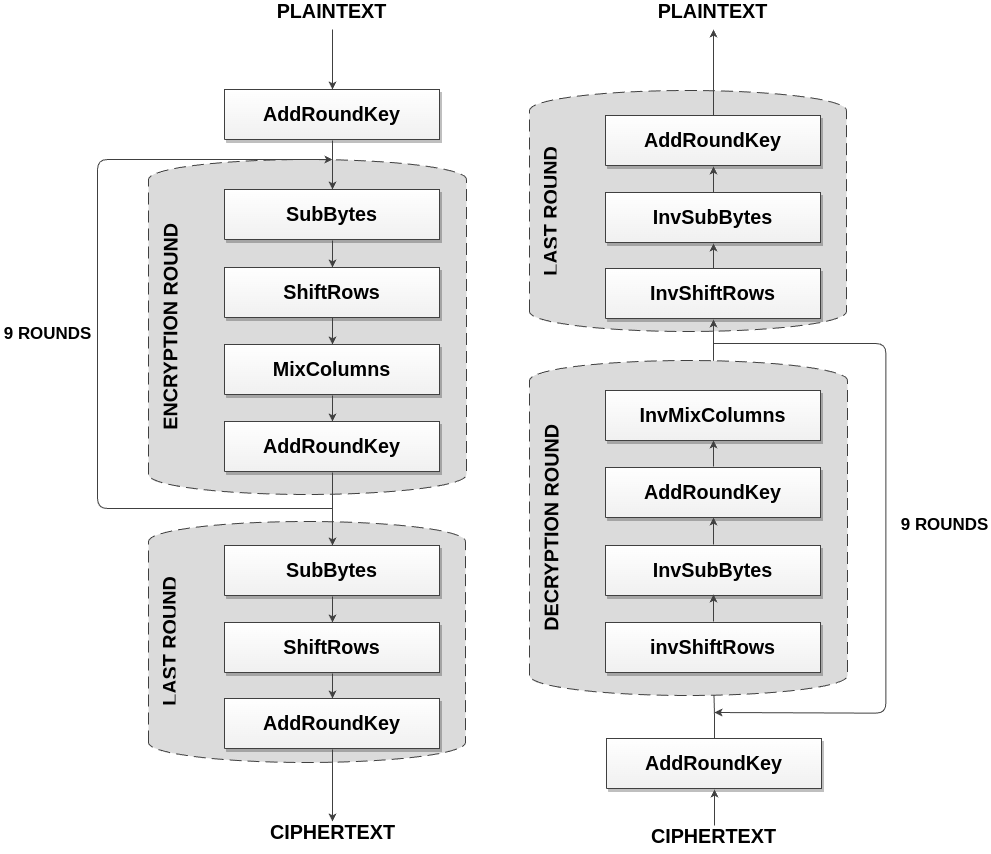
\includegraphics[width= 0.8\textwidth]{figure_5.2}\\
\caption{ (left) AES encryption algorithm, (right) AES decryption algorithm }
\label{fig:figure_5.2}
\end{figure}
AES consists of four sub-functions:\\
\underline{For encryption:}
\begin{outline}
\1 SubBytes
\1 ShiftRows
\1 MixColumns
\1 AddRoundKey
\end{outline}

\noindent\underline{For decryption:}
\begin{outline}
\1 InvSubBytes
\1 InvShiftRows
\1 InvMixColumn
\1 InvAddRoundKey
\end{outline}

Before elaborating on these functions, we must first introduce a convention. The algorithm's input is a block of 128 bits, which, after being subjected to several transformations, results in the output. During these transformations, the block is referred to as the "state".

%  fig 5.3
\begin{figure}
\centering
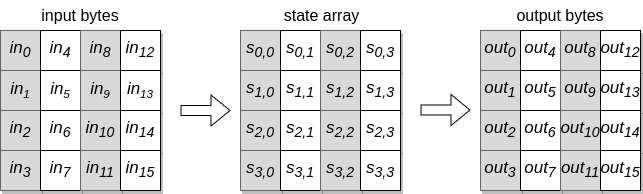
\includegraphics[width= 0.8\textwidth]{figure_5.3}\\
\caption{ AES input bytes, state array, and output bytes}
\label{fig:figure_5.3}
\end{figure}

The subscripts in Figure \ref{fig:figure_5.3} denote the position of the byte in the block. The usage of the terms "row" and "column" should be interpreted with this convention in mind.

The SubBytes operation replaces the value of each byte in the block. The mapping of values is performed using the mathematical process. The calculation of the transformation consists of two parts. The first part is the calculation of the multiplicative inverse in the field $GF(2^8)$. The second part is the calculation of the inverse of the affine transformation. The calculation of the multiplicative inverse is presented in Figure \ref{fig:figure_5.4}. The individual operations involved are defined:\\

\begin{equation}
\delta \equiv \begin{bmatrix}
1  & 0  & 1  & 0  & 0  & 0  & 0  & 0 \\
1  & 1  & 0  & 1  & 1  & 1  & 1  & 0  \\ 
1  & 0  & 1  & 0  & 1  & 1  & 0  & 0  \\
1  & 0  & 1  & 0  & 1  & 1  & 1  & 0  \\
1  & 1  & 0  & 0  & 0  & 1  & 1  & 0  \\
1  & 0  & 0  & 1  & 1  & 1  & 1  & 0  \\
0  & 1  & 0  & 1  & 0  & 0  & 1  & 0  \\
0  & 1  & 0  & 0  & 0  & 0  & 1  & 1  \\
\end{bmatrix}
\cdot
\begin{bmatrix}
x7 \\ x6 \\ x5 \\ x4 \\ x3 \\ x2 \\ x1 \\ x0 \\ 
\end{bmatrix}
=
\begin{bmatrix}
x7\oplus x5  \\
x7\oplus x6\oplus x4\oplus x3\oplus x2\oplus x1 \\
x7\oplus x5\oplus x3\oplus x2 \\
x7\oplus x5\oplus x3\oplus x2\oplus x1 \\
x7\oplus x6\oplus x2\oplus x1 \\
x7\oplus x4\oplus x3\oplus x2\oplus x1 \\
x6\oplus x4\oplus x1 \\
x6\oplus x1\oplus x0 \\
\end{bmatrix}
\\\\
\end{equation}

\begin{equation}
\delta ^-1 \equiv 
\begin{bmatrix}
1  & 1  & 1  & 0  & 0  & 0  & 1  & 0 \\
0  & 1  & 0  & 0  & 0  & 1  & 0  & 0 \\
0  & 1  & 1  & 0  & 0  & 0  & 1  & 0 \\
0  & 1  & 1  & 1  & 0  & 1  & 1  & 0 \\
0  & 0  & 1  & 1  & 1  & 1  & 1  & 0 \\
1  & 0  & 0  & 1  & 1  & 1  & 1  & 0 \\
0  & 0  & 1  & 1  & 0  & 0  & 0  & 0 \\
0  & 1  & 1  & 1  & 0  & 1  & 0  & 1 \\
\end{bmatrix}
\cdot
\begin{bmatrix}
x7 \\ x6 \\ x5 \\ x4 \\ x3 \\ x2 \\ x1 \\ x0 \\ 
\end{bmatrix}
=
\begin{bmatrix}
x7\oplus x6\oplus x5\oplus x1  \\
x6\oplus x2 \\
x6\oplus x5\oplus x1  \\
x6\oplus x5\oplus x4\oplus x2\oplus x1  \\
x5\oplus x4\oplus x3\oplus x2\oplus x1  \\
x7\oplus x4\oplus x3\oplus x2\oplus x1  \\
x5\oplus x4 \\
x6\oplus x5\oplus x4\oplus x2\oplus x0  \\
\end{bmatrix}\\
\end{equation}\\

% fig 5.4
\begin{figure}
\centering
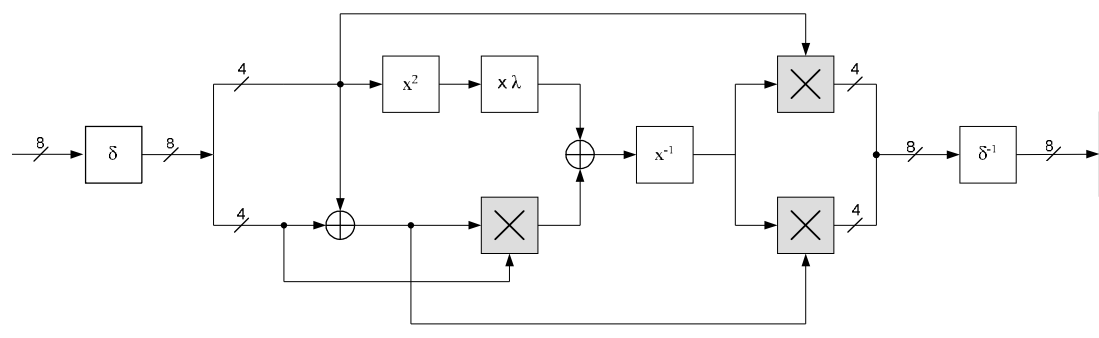
\includegraphics[width= 0.8\textwidth]{figure_5.4}\\
\caption{ Multiplicative inverse in $GF(2^8)$ }
\label{fig:figure_5.4}
\end{figure}

\begin{equation}
x^2 \equiv
\begin{bmatrix}
x3 \\
x3\oplus x2 \\
x2\oplus x1 \\
x3\oplus x1\oplus x0 \\
\end{bmatrix}
\end{equation}

\begin{equation}
x\lambda \equiv
\begin{bmatrix}
x2\oplus x0 \\
x3\oplus x2\oplus x1\oplus x0 \\
x3 \\
x2 \\
\end{bmatrix}\\
\end{equation}\\

\noindent
Additionally, the definition of multiplication is:\\
\begin{equation}
% \begin{split}
% \begin{aligned}
x\cdot y \equiv\\
\begin{bmatrix}
[(x3\oplus x1)(y3\oplus y1)]\oplus [(x2\oplus x0)(y3\oplus y1)]\oplus [(x3\oplus x1)(y2\oplus y0)]\oplus \\\oplus  (x1\cdot y1)\oplus (x0\cdot y1)\oplus (x1\cdot y0) \\\\
[(x3\oplus x1)(y3\oplus y1)]\oplus [(x2\oplus x0)(y2\oplus y0)]\oplus (x1\cdot y1)\oplus (x0\cdot y0) \\\\
(x1\cdot y1)\oplus (x0\cdot y1)\oplus (x1\cdot y0)\oplus (x3\cdot y3)\oplus (x2\cdot y3)\oplus (x3\cdot y2)\oplus (x2\cdot y2) \\\\
(x1\cdot y1)\oplus (x0\cdot y0)\oplus (x3\cdot y3)\oplus (x2\cdot y3)\oplus (x3\cdot y2) \\\\
\end{bmatrix}\\
% \end{split}
% \end{aligned}
\end{equation}\\

\noindent
Finally, we have the value mapping for the multiplicative inverse in $GF(2^4)$:\\
\begin{equation}
\begin{split}
x^{-1}(0000)= 0000, x^{-1}(0001)= 0001, x^{-1}(0010)= 0011, x^{-1}(0011)= 0010\\
x^{-1}(0100)= 1111, x^{-1}(0101)= 1100, x^{-1}(0110)= 1001, x^{-1}(0111)= 1011\\
x^{-1}(1000)= 1010, x^{-1}(1001)= 0110, x^{-1}(1010)= 1000, x^{-1}(1011)= 0111\\
x^{-1}(1100)= 0101, x^{-1}(1101)= 1110, x^{-1}(1110)= 1101, x^{-1}(1111)= 0100\\  
\end{split}
\end{equation}\\


The calculation of the inverse affine transformation takes one byte as input and computes the following operation:\\

\begin{equation}
AT^{-1} \equiv
\begin{bmatrix}
0  & 1  & 0  & 1  & 0  & 0  & 1  & 0 \\
0  & 0  & 1  & 0  & 1  & 0  & 0  & 1 \\
1  & 0  & 0  & 1  & 0  & 1  & 0  & 0 \\
0  & 1  & 0  & 0  & 1  & 0  & 1  & 0 \\
0  & 0  & 1  & 0  & 0  & 1  & 0  & 1 \\
1  & 0  & 0  & 1  & 0  & 0  & 1  & 0 \\
0  & 1  & 0  & 0  & 1  & 0  & 0  & 1 \\
1  & 0  & 1  & 0  & 0  & 1  & 0  & 0 \\
\end{bmatrix}
\cdot
\begin{bmatrix}
x7 \\
x6 \\
x5 \\
x4 \\
x3 \\
x2 \\
x1 \\
x0 \\
\end{bmatrix}
+
\begin{bmatrix}
0 \\
0 \\
0 \\
0 \\
0 \\
1 \\
0 \\
1 \\
\end{bmatrix}\\
\end{equation}\\

where $x_n$ is the n\ts{th} bit of the input byte. ShiftRows performs a one-byte rotation of the \nth{2} row, a two-byte rotation of the \nth{3} row, and a three-byte rotation of the \nth{4} row. 
 MixColumns multiplies each column by the matrix:\\

\begin{equation}\label{eq:mixcolumns}
\begin{bmatrix}
02 & 03 & 01 & 01 \\
01 & 02 & 03 & 01 \\
01 & 01 & 02 & 03 \\
03 & 01 & 01 & 02 \\
\end{bmatrix}_{10}\\
\end{equation}\\

\noindent
and the result replaces the initial column. Finally, the AddRoundKey performs bitwise XOR of the block and the round key.
The decryption operations execute the inverse process. Thus, the InvSubBytes performs the inverse substitution of the value of each byte. To calculate the inverse value, the byte first undergoes an affine transformation:\\

\begin{equation}
AT  \equiv
\begin{bmatrix}
1  & 0  & 1  & 0  & 0  & 0  & 0  & 0  &  \\
1  & 1  & 0  & 1  & 1  & 1  & 1  & 0  &  \\
1  & 0  & 1  & 0  & 1  & 1  & 0  & 0  &  \\
1  & 0  & 1  & 0  & 1  & 1  & 1  & 0  &  \\
1  & 1  & 0  & 0  & 0  & 1  & 1  & 0  &  \\
1  & 0  & 0  & 1  & 1  & 1  & 1  & 0  &  \\
0  & 1  & 0  & 1  & 0  & 0  & 1  & 0  &  \\
0  & 1  & 0  & 0  & 0  & 0  & 1  & 1  &  \\
\end{bmatrix}
\cdot
\begin{bmatrix}
x7 \\
x6 \\
x5 \\
x4 \\
x3 \\
x2 \\
x1 \\
x0 \\
\end{bmatrix}
+
\begin{bmatrix}
1 \\
1 \\
0 \\
0 \\
0 \\
1 \\
1 \\
0 \\
\end{bmatrix}\\
\end{equation}\\

\noindent
and then through an inverse multiplication in $GF(2^8)$.
The InvShiftRows performs the same rotations in the opposite direction (right), and the InvMixColumns multiplies by the inverse matrix of MixColumns:\\

\begin{equation} \label{eq:invmixcolumns}
\begin{bmatrix}
14 & 11 & 13 & 09 \\
09 & 14 & 11 & 13 \\
13 & 09 & 14 & 11 \\
11 & 13 & 09 & 14 \\
\end{bmatrix}_{10}\\
\end{equation}\\

\noindent
and the InvAddRoundKey is the same as the AddRoundKey.

In the key generation process, a matrix of constant values, called $Rcon$, is involved which is defined as: \\

\begin{equation} \label{eq:rcon}
    Rcon \equiv \begin{bmatrix}
01 & 02 & 04 & 08 & 10 & 20 & 40 & 80 & 1B & 36 \\
00 & 00 & 00 & 00 & 00 & 00 & 00 & 00 & 00 & 00 \\
00 & 00 & 00 & 00 & 00 & 00 & 00 & 00 & 00 & 00 \\
\end{bmatrix}_{16}\\
\end{equation}

\noindent
Each column of this matrix participates in the corresponding round key generation. (the \nth{1} in the \nth{1} round, the \nth{2} in the \nth{2}, etc.).
The key generation process is as follows:
To generate the first column of the new key, the last column of the previous key is selected, and a RotWord (see Figure \ref{fig:figure_5.5}) is performed. Then, each byte of the column undergoes the SubBytes process, and finally, this column, along with the \nth{1} column of the previous key and the corresponding column of the Rcon matrix, undergo bitwise XOR. The resulting column is the \nth{1} column of the new key.

 % fig 5.5
\begin{figure}
\centering
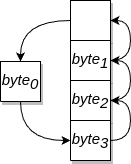
\includegraphics[width= 0.2\textwidth]{figure_5.5}\\
\caption{ The RotWord operation}
\label{fig:figure_5.5}
\end{figure}


The value of the \nth2 column is the result of the bitwise XOR of the \nth{2} column of the previous key with the \nth{1} column of the new key, the \nth{3} column's value is the result of the bitwise XOR of the \nth{3} column of the previous key with the \nth{2} column of the new key, and the \nth{4} column's value is the result of the bitwise XOR of the \nth{4} column of the previous key with the \nth{3} column of the new key. This process is repeated 10 times to produce 10 keys, one for each encryption round. The keys generated are passed to the AddRoundKey of the corresponding round. It is noteworthy that in decryption, the keys are provided in the reverse order compared to encryption.

\subsubsection*{Design Decisions}
Various parameters need to be taken into account, before commencing the design and implementation of this peripheral. Since the peripheral will operate as a slave of a processor, the interfaces between them, the communication protocol, and the individual technical details must be first defined.

In a processing system, the processor undertakes various tasks. Therefore, peripherals should be designed to operate with waiting states. In the case of CBC-AES-128, the peripheral should be in a waiting state until the processor provides it with the next input or command. Additionally, when an operation is completed and there is output available for the processor, the peripheral should have a way to notify the processor and wait until the processor consumes the peripheral's output.

For the communication protocol between the peripheral and the processor, both control signals driven by the processor and status signals driven by the peripheral are needed. These signals are designed, and their behavior is defined in a way that facilitates straightforward hardware design and straightforward management from the software side.

An important design decision is choosing the data transfer method between the peripheral and the memory. Many options exist, such as DMA, the peripheral switching between master and slave modes in the main bus, or direct access to the processor's registers (a Microblaze feature provided by Xilinx, called FSL, Fast Simplex Link). Ultimately, because the system is not multipacket, the processor does not process many packets simultaneously, and therefore there is no benefit in a peripheral taking over the data transfer, as during the data transfer, the processor will be blocked in a waiting state. Thus, the design decision is that the data transfer will be performed by the processor.

Finally, regarding the means of the peripheral notifying processor, there exist two options, polling and using interrupts. The polling method is implemented since due to the lack of multipacketing, the processor would be inactive while waiting for an interrupt.


\subsubsection*{Hardware Design}
The hardware design is organized hierarchically. At the lowest level, the internal operations of AES (ShiftRows, SubBytes, MixColumns, AddRoundKey) are implemented. These are used to implement the unit that executes one round of AES and another unit that executes one round of the key expansion. The complete key expansion unit is then implemented. Finally, at the top level, these subcomponents are integrated to implement the complete AES in CBC mode. Next, we elaborate on the hardware designs, in a bottom-up approach.

The implementation of ShiftRows and InvShiftRows is simply a permutation of their input bytes. The unit implementing the SBOX and its inverse (InvSBOX), receives a signal called EncDec which indicates whether the unit will operate in encryption or decryption mode. This design choice is made with resource reuse of the inverse multiplication $GF(2^8)$ in mind in order to optimize the area utilization of these components. The affine transform, inverse affine transform, and multiplicative inverse are designed using logic gates that directly implement their equations. Figure \ref{fig:figure_5.6} presents the block diagram of the unit. Due to the combined implementation of SBOX and InvSBOX, the implementation of SubBytes and InvSubBytes is also combined in a unit that accepts an EncDec signal that is passed down to these operations. The block diagram of the unit of SubBytes and InvSubBytes is shown in Figure \ref{fig:figure_5.7}.

 % fig 5.6
\begin{figure}[H]
\centering
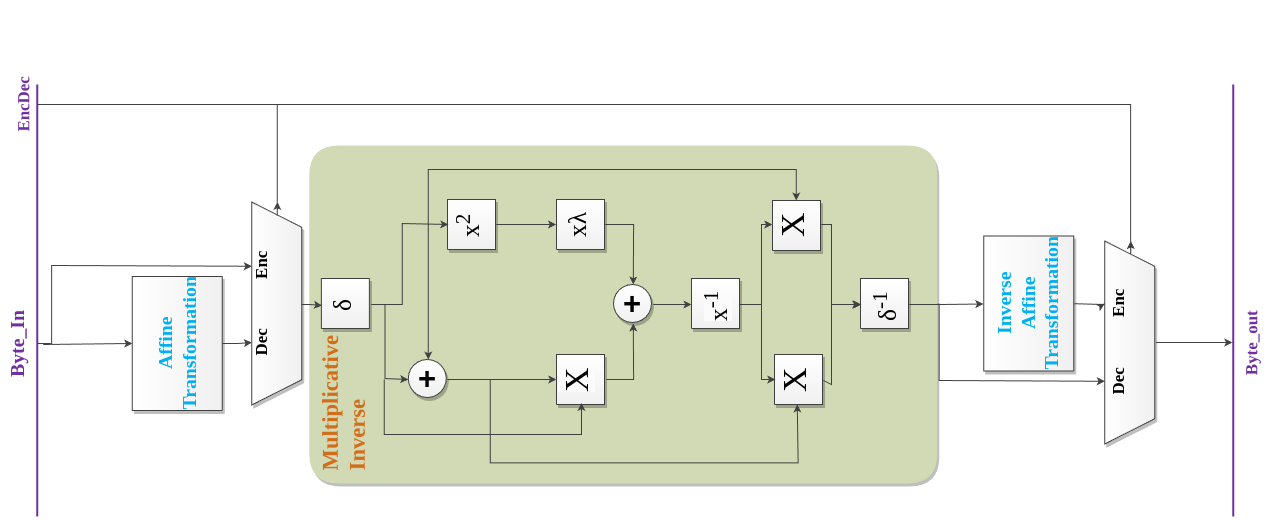
\includegraphics[width = 1.4\textwidth, angle=270,origin=c]{figure_5.6}\\
\caption{ Combined implementation of SBOX and InvSBOX }
\label{fig:figure_5.6}
\end{figure}


% fig 5.7
\begin{figure}
\centering
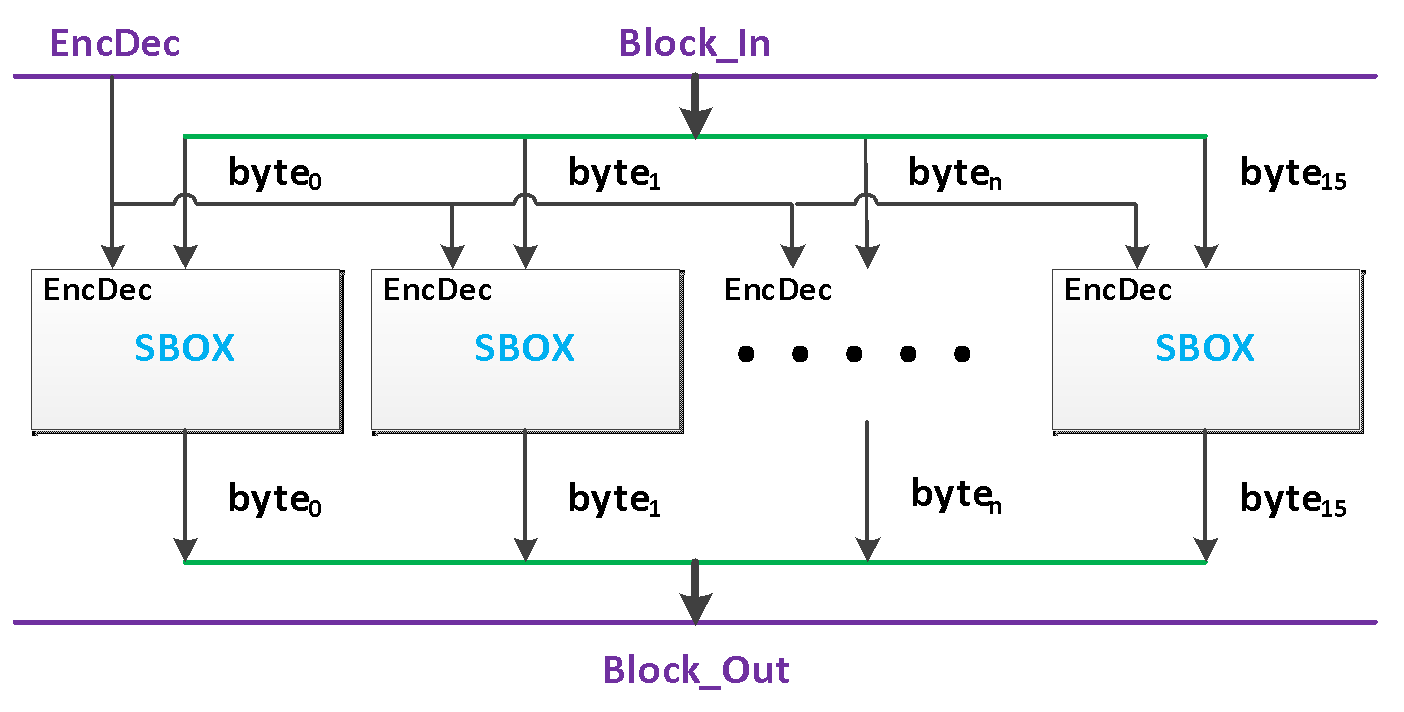
\includegraphics[width= 0.8\textwidth]{figure_5.7}\\
\caption{ Combined implementation of SubBytes and InvSubBytes }
\label{fig:figure_5.7}
\end{figure}

The operations MixColumns and InvMixColumns are implemented in a combined unit. The selection of the operation is specified using an EncDec signal. Because each column is processed independently of other columns, 4 subunits named MixOneColumn, one per column, are implemented to exploit parallelism and thus reduce latency. The block diagram of the combined MixColumns and InvMixColumns unit is presented in Figure \ref{fig:figure_5.8}.

% fig 5.8
\begin{figure}
\centering
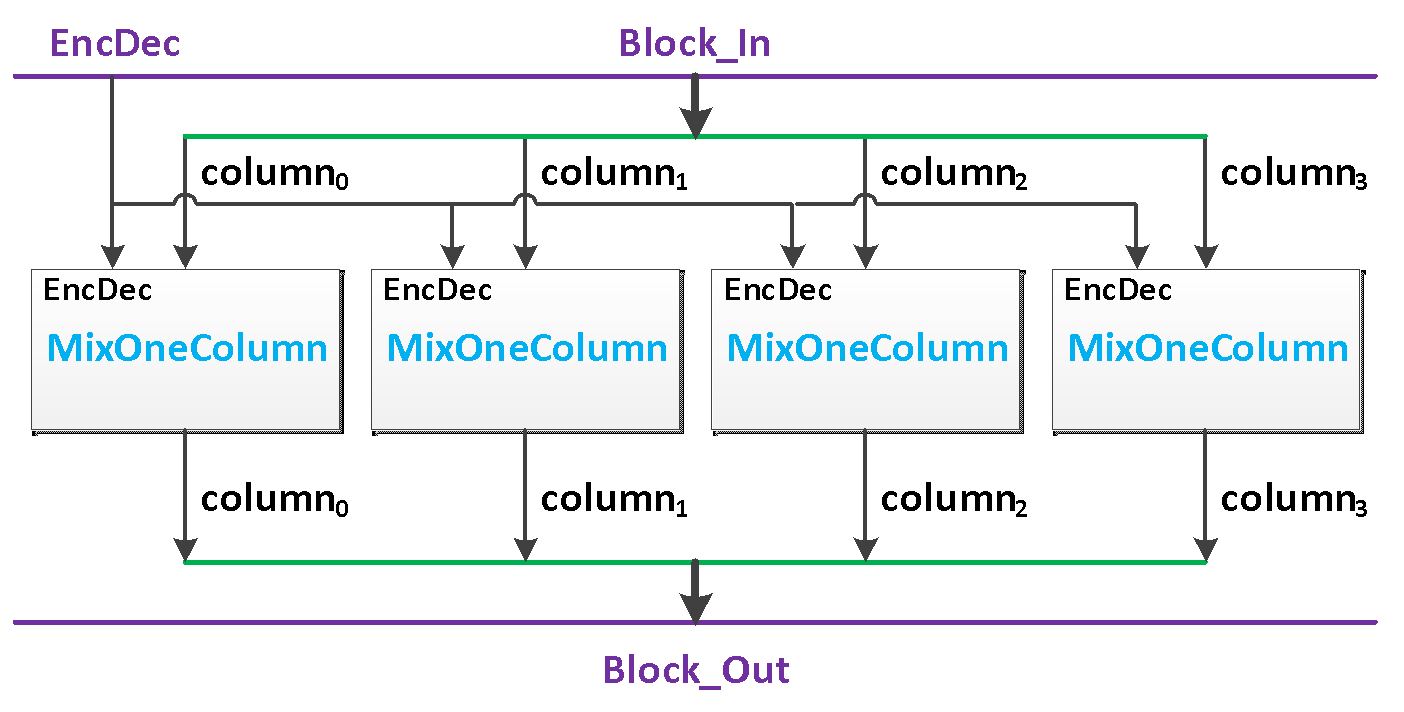
\includegraphics[width= 0.8\textwidth]{figure_5.8}\\
\caption{   Combined implementation of MixColumns and InvMixColumns}
\label{fig:figure_5.8}
\end{figure}

In each MixOneColumn, the column is multiplied by the matrix ~\ref{eq:mixcolumns} during encryption and by the matrix ~\ref{eq:invmixcolumns} during decryption. We observe that each byte of the column must be multiplied by the numbers $02$ and $03$ for encryption and by $14$, $11$, $13$, and $09$ for decryption. Thus, a unit named XTimes is created, which takes one byte as input and outputs its multiples of 2, 3, 9, 11, 13, and 14. The appropriate additions of the multiples are performed, and the final results are placed in the corresponding bytes of the output column. The implementation of MixOneColumn is presented in Figure \ref{fig:figure_5.9}. In this figure, to distinguish the outputs of XTimes, a suffix with the byte number is used (the signal x2\_0 means twice byte\ssc{0}, x14\_3 means 14 times byte\ssc{3}, and so on).

% fig 5.9
\begin{figure}[H]
\centering
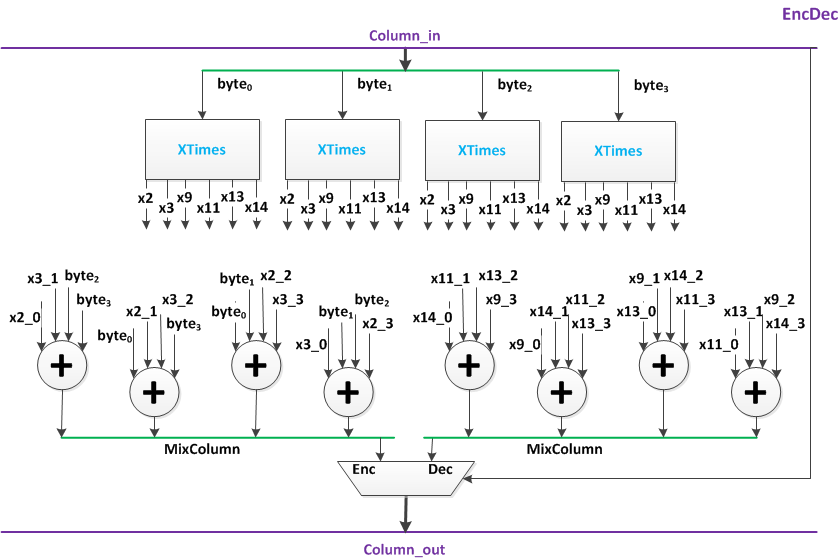
\includegraphics[width= 0.8\textwidth]{figure_5.9}\\
\caption{ Implementation of MixOneColumn}
\label{fig:figure_5.9}
\end{figure}

The implementation of XTimes is presented in Figure \ref{fig:figure_5.10}. The individual operations are characterized by the following equations: \\

\begin{equation}
\begin{split}
&3x=2x\oplus x,\\
&4x=2\cdot 2x,\\
&8x=2\cdot 4x,\\
&9x=x\oplus8x,\\
&10x=2x\oplus 8x,\\
&11x=10x\oplus x,\\
&12x=10x\oplus 2x,\\
&13x=12x\oplus x,\\
&14x=12x\oplus2x \\
\end{split}
\end{equation}\\

% fig 5.10
\begin{figure}
\centering
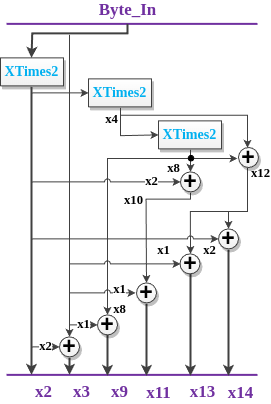
\includegraphics[width= 0.4\textwidth]{figure_5.10}\\
\caption{ Implementation of XTimes }
\label{fig:figure_5.10}
\end{figure}


In Figure \ref{fig:figure_5.11}, the unit for computing the double of XTimes, named XTimes2 is illustrated. This operation takes place in the $GF(2^8)$ field and is defined as follows: For the input byte, a left shift is performed first. If the MSbit of the input byte is 0, then the shift does not overflow, and the output is given by the shifted byte. Otherwise, if there is overflow, the value $1B_{16}$ must be added (via XOR) to the shifted byte.

% fig 5.11
\begin{figure}
\centering
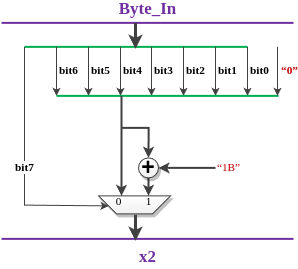
\includegraphics[width= 0.5\textwidth]{figure_5.11}\\
\caption{ Implementation of XTimes2 }
\label{fig:figure_5.11}
\end{figure}


The last unit in an AES round is the AddRoundKey, which is simply a bitwise XOR between the block and the current round key. The key is provided as input, and ultimately, AddRoundKey is a bitwise XOR of length 128 bits.

Finally, combining the above units, a unit for computing a round of AES-128 is implemented. Its inputs are the input block, the key of the current round, the EncDec signal for selecting encryption or decryption mode, and a LastRound signal indicating if the operation is currently executing the last AES round. LastRound is needed because the last round of AES-128 differs from the preceding 9 rounds. The output of the unit is the processed block. The block diagram of the design is presented in Figure \ref{fig:figure_5.12}. The differences between encryption and decryption are (as shown in Figure \ref{fig:figure_5.2}):
\begin{outline}[enumerate]
\1 Execution of ShiftRows versus execution of InvShiftRows
\1 Execution of SubBytes  versus execution of InvSubBytes
\1 Execution of MixColumns  versus execution of InvMixColumns
\1 Execution of AddRoundKey after MixColumns in encryption, and vice versa for decryption.
\end{outline}
The first difference is implemented using a MUX, which selects between the output of ShiftRows or InvShiftRows based on the EncDec signal. The second and third differences are already implemented within the common units of SubBytes and MixColumns respectively, using the EncDec signal. The fourth difference is implemented using two AddRoundKey units, one placed before MixColumns and one placed after. When in encryption mode, the first AddRoundKey is bypassed using a MUX, while the second one is used. In decryption, the second one is bypassed with a MUX while the first one is used.

The difference in the final rounds of encryption and decryption from the other 9 is (as shown in Figure 5.2) that the MixColumns and InvMixColumns operations are not performed respectively. Because these two operations are implemented in one unit, only one bypass MUX is needed with the LastRound signal as the selection signal.

% fig 5.12
\begin{figure}
\centering
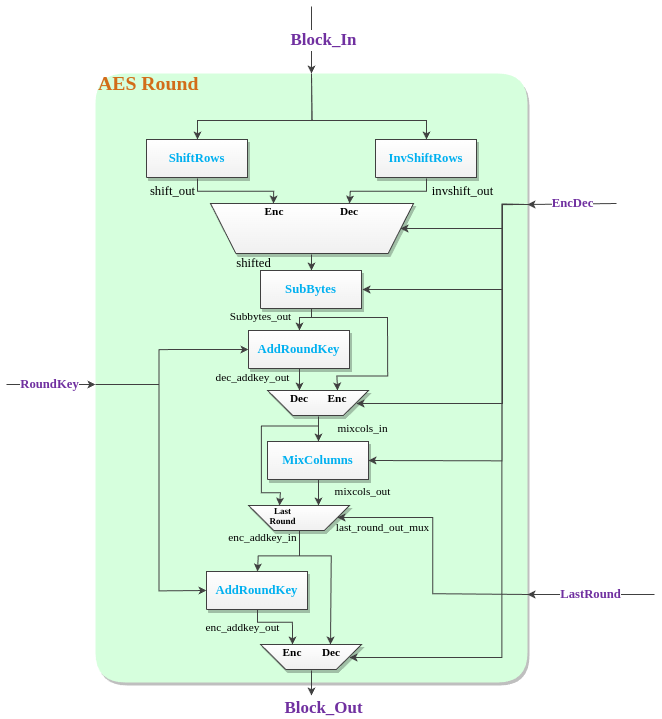
\includegraphics[width= 1\textwidth]{figure_5.12}\\
\caption{  Implementation of one round of AES-128 }
\label{fig:figure_5.12}
\end{figure}

For the calculation of the round keys, first, a unit named KeyScheduleRound is implemented for computing the next round key. The key calculation is identical for encryption and decryption, with the only difference being that during decryption, the keys are provided to the AES rounds in the reverse order from the order in which they are calculated. This difference is managed at a higher level of the design. The block diagram of the KeyScheduleRound is presented in Figure \ref{fig:figure_5.13}.

The KeyScheduleRound unit takes as inputs the key of the previous round and the Rcon value corresponding to the current round and outputs the key generated for the current round. In the design, 4 SBOX units are used, each for each of the 4 bytes of the last column of the input key. Because the inverse operation InvSBOX is not needed, a separate SBOX unit is implemented, which performs only the calculations for multiplicative inverse and inverse affine transform, to save on area utilization.

% fig 5.13
\begin{figure}
\centering
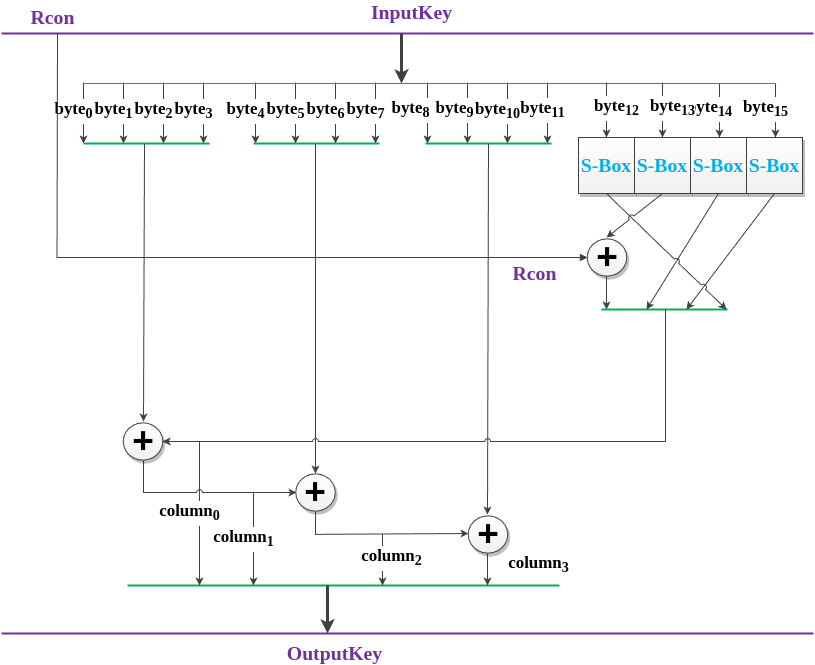
\includegraphics[width= 0.8\textwidth]{figure_5.13}\\
\caption{ Implementation of one round of AES-128 Key Scheduler }
\label{fig:figure_5.13}
\end{figure}

The computations executed are as follows: first, the substitution through the SBOX of the last column of the input key is performed, and the result undergoes a RotWord, which is simply a permutation of the bytes. After RotWord, a bitwise XOR with the value of Rcon is performed. From Figure \ref{eq:rcon}, we observe that the last 3 bytes of each column of Rcon are zero, so they do not affect the bitwise XOR. Thus, only the first byte of Rcon is needed as input, and a bitwise XOR of 8 bits instead of 32 bits is sufficient. The first column of the output key is the processed last column of the input. The second output column is calculated with a bitwise XOR between the first input column and the processed last input column, the third with a bitwise XOR of the second output column with the second input column, and the fourth with the third output and the third input column.

Using KeyScheduleRound, the unit for computing all round keys, named KeyScheduler, is implemented. Its block diagram is presented in Figure \ref{fig:figure_5.14}. Its inputs are the initial key, a round counter indicating the current round, and the signal FirstRound indicating that we are in the first round. The output provides the current round key at any given time. The unit contains a KeyScheduleRound subunit and an Rcon subunit which takes as input the round counter and outputs the first byte of the corresponding column of Rcon (since the others are $'00'$) and feeds this value to the KeyScheduleRound.

% fig 5.14
\begin{figure}
\centering
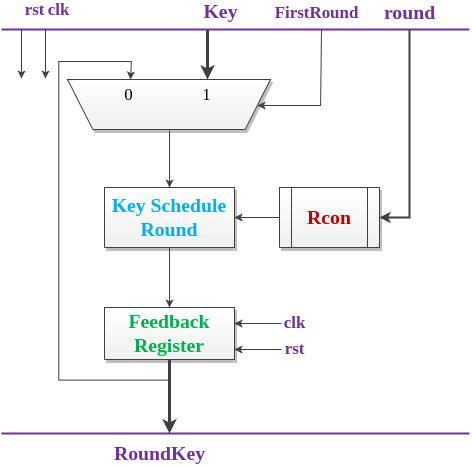
\includegraphics[width= 0.6\textwidth]{figure_5.14}\\
\caption{ Implementation of the AES-128 Key Scheduler }
\label{fig:figure_5.14}
\end{figure}


The value of the first derived key depends on the value of the initial key while the value of any other derived key depends on the directly preceding derived key. The FirstRound signal helps differentiate between the two scenarios. It is used to route either the initial key or the preceding derived key through the feedback loop back as input to the KeyScheduleRound unit.

Finally, the peripheral of CBC-AES-128 is implemented. Its block diagram is presented in Figure \ref{fig:figure_5.15}. Its inputs are:
\begin{outline}
    \1 Block\_in: the current message block
    \1 IV: the initialization vector
    \1 Key: the cryptographic key
    \1 Start\_new: a control signal denoting an instruction for a new encryption/decryption operation
    \1 Next\_block: a control signal indicating that the next input block is present at the Block\_in
    \1 EncDec: a control signal for selecting between encryption and decryption operations
    \1 clk: the system's clock signal
    \1 rst: the system's reset signal
\end{outline}
As outputs, the peripheral provides the output block and a control signal named 'ready' indicating the end of block processing, i.e., that the output block is ready.

In Figure \ref{fig:figure_5.15} the colored area on the left outlines the parts that implement the CBC operation. The part in the middle is the AES operation, and the part on the right is the key generation operation. In the bottom right, the peripheral's control circuit is presented, alongside its input and output signals.

The CBC implementation uses two bitwise XORs, one applied at the input block before it is passed to the AES operation and one applied at the output of the AES operation. The first XOR gets selected by a MUX when in encryption mode, while the second XOR is selected in decryption mode. The second input of both XORs is determined based on the combination of the current block number and if the operation is encryption or decryption. When we are processing the first block, the IV is provided to the XORs. For any other block, if we are in encryption mode, the value of the previous AES output is provided, while if in decryption mode, the value provided is the previous input block. These options are implemented with the appropriate placement of registers, MUXes, and the needed control signals managed by the control circuit.

% fig 5.15
\begin{figure}
\centering
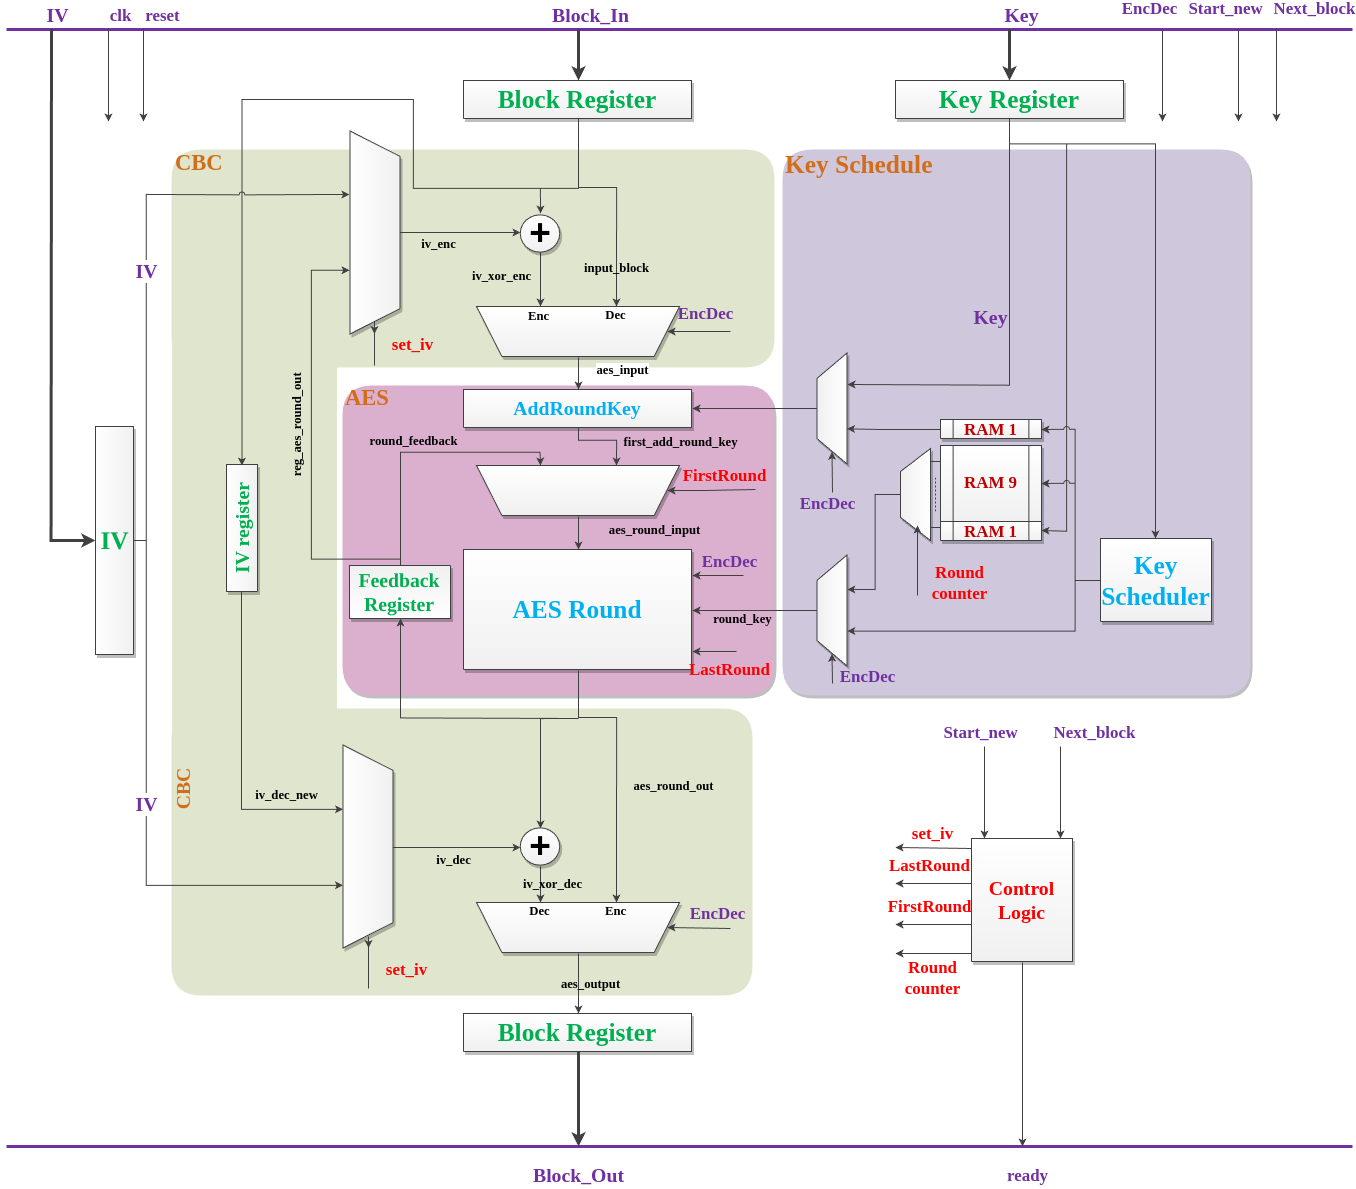
\includegraphics[width= 0.8\textwidth]{figure_5.15}\\
\caption{ Implementation of CBC-AES-128 }
\label{fig:figure_5.15}
\end{figure}


The AES part first needs to perform an AddRoundKey to the input before continuing with the 10-round processing, as shown in Figure \ref{fig:figure_5.2}. The 10 AES rounds are implemented by using a feedback loop around the AES Round unit. The signal FirstRound selects which value will be used in the AES Round, either the result of the AddRoundKey or the previous output via feedback.

The core of the key generation operation is a KeyScheduler unit. When in encryption mode, where the keys must be provided in the order they are generated, the KeyScheduler directly provides its output to the AES Round, and the initial AddRoundKey is given the initial key from the input. In decryption mode, where the keys must be provided in the reverse order of the order they get generated, the last key must be given to the initial AddRoundKey, which requires the computation and storing of all the keys in advance. For this purpose, 11 registers are used as the key storage. The first 10 registers are populated by the KeyScheduler starting from the last register and in reverse order. This way the keys are stored in reverse order and are mapped correctly with their respective rounds. The initial input key is placed in the last (\nth{11}) register. Finally, the first register is connected directly to the AddRoundKey to provide the last derived key, while the other registers are selected by a MUX based on the round counter to be routed to the AES Round.

The control circuit receives the signals Start\_new and Next\_Block and provides the output signal ready and the internal control signals set\_iv (used for IV selection), LastRound, FirstRound, and Round\_counter, which is the counter indicating the current round. The control circuit is described by the FSM shown in Figure ~\ref{fig:figure_5.16}:

% fig 5.16
\begin{figure}
\centering
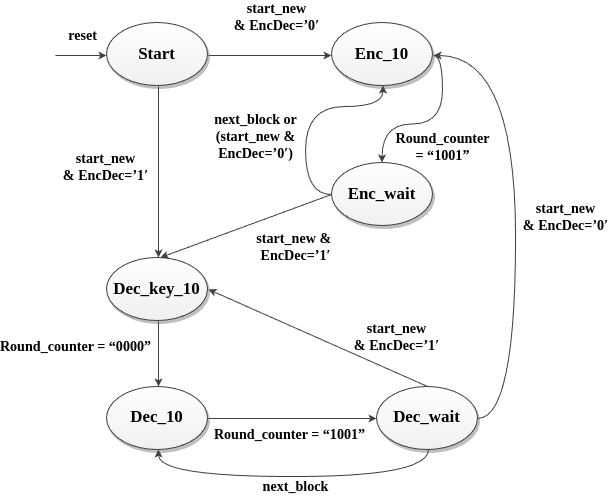
\includegraphics[width= 0.8\textwidth]{figure_5.16}\\
\caption{ The control FSM of CBC-AES-128 }
\label{fig:figure_5.16}
\end{figure}


Upon each reset, the FSM transitions to the initial Start state, where it waits for a start\_new signal. When start\_new arrives and depending on the value of the EncDec signal, it transitions to either encryption mode (EncDec='0') or decryption mode (EncDec='1'). Before a start\_new signal is issued, the key, the IV, and the first block of the message must be already provided at the module's inputs.

Encryption mode operates using two states. In the state Enc\_10, the 10 encryption rounds of AES are executed, and when finished it transitions to the Enc\_Wait state, where the peripheral waits. The transition between the two is implemented using a comparator that compares the Round\_Counter with the value "1001" (counting starts from 0, so a total of 10 rounds are counted). While in Enc\_Wait state, the peripheral waits for either the next block of the same message, indicated by the next\_block signal, or the start of a new message indicated by the start\_new signal. When a next\_block is received, the FSM returns back to Enc\_10 to process the new block. If start\_new arrives, the next FSM state depends on the value of EncDec. If  EncDec is '0', the FSM transitions to the Enc\_10  state in order to encrypt the first block of the new message, while if EncDec is '1', the FSM transitions to the Dec\_Key\_10 state, which is the first stage of the decryption operation.

In decryption mode, we have three states: Dec\_Key\_10, where all the keys first are generated and stored, Dec\_10, where the 10 decryption rounds of AES are executed, and Dec\_Wait, which is a waiting state that serves a similar purpose to Dec\_Wait. The keys must be generated once for every new message, thus Dec\_Key\_10 only takes place once at the start of the decryption process and there is no need to regenerate them on the arrival of every new block since the keys are kept in the key registers.

In Dec\_Key\_10, the Round\_Counter starts from the value "1001" so that the appropriate key registers are selected and traversed in reverse order. When Round\_Counter reaches 0, the decryption of the first block can commence by transitioning to state Dec\_10. The Round\_Counter gets increased in every round, and, after executing the 10 decryption rounds, Round\_Counter is "1001". At this point the FSM transitions to the waiting state Dec\_Wait. Dec\_Wait is identical to Enc\_Wait except from the fact that state transitions differ.

\subsection{HMAC-SHA1-96}
\subsubsection*{Algorithm Specification}
HMAC-SHA1-96 is a MAC algorithm that utilizes the cryptographic hash algorithm SHA1. The number 96 in the name indicates how many bits of the output are used. The mathematical formulation of HMAC is:

\begin{equation}
HMAC(K, text)_t=H[(K_0\oplus opad) || H((K_0\oplus ipad) || text)]_t
\end{equation}

\noindent
where:
\begin{outline}
\1 $text$ represents the input text,
\1 $H$ is the hash function used (in this case it is SHA1),
\1 $K$ is the key,
\1 $K_0$ is the key after preprocessing,
\1 $ipad$ is the repetition of the byte $[36]_{16}$, with a total size equal to the block size of the hash function,
\1 $opad$ is the repetition of the byte $[5C]_{16}$, with a total size equal to the block size of the hash function,
\1 $||$ denotes concatenation,
\1 $t$ is the size of the received output.
\end{outline}\\

\noindent
Figure \ref{fig:figure_5.17}, presents the HMAC operation schematically.

% fig 5.17
\begin{figure}[H]
\centering
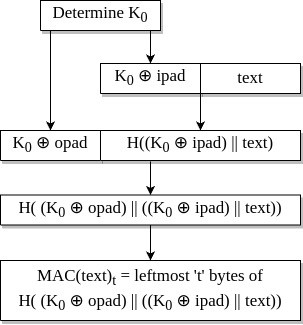
\includegraphics[width= 0.5\textwidth]{figure_5.17}\\
\caption{ The HMAC algorithm}
\label{fig:figure_5.17}
\end{figure}

HMAC has a preprocessing phase, where the value $K_0$ gets generated from the key $K$. The process differs depending on the size of key $K$ and the block size of $H$. When the size of $K$ matches the block size of $H$, $K$ simply takes the value of $K_0$. If the size of $K$ is smaller than the size of $H$, a padding of '0' bits is applied, while if larger, $K$ is first transformed through $H$ to produce $K_0$.

The SHA1 algorithm has an output size of 160 bits. It divides its input into 512-bit blocks and padding is applied for inputs whose size is not a multiple of 512 bits. It executes 80 iterations to process each input block. The algorithm is described in Algorithm \ref{alg:hmac_pre}, where $N$ is the number of input blocks, $M^i$ is the $i\ssc{th}$ input block and:

\begin{equation}
f_t(x,y,z) \equiv 
\begin{cases}
      M_t^{(i)} & 0 \leq t \leq 15\\
      ROTL^1(W_(t-3)\oplus W_(t-8)\oplus W_(t-14)\oplus W_(t-16)) & 16 \leq t \leq 79
\end{cases} \end{equation} \label{eq:f_t}


\begin{equation}
K_t \equiv 
\begin{cases}
    5a827999 & 0 \leq t \leq 19\\ 
    6ed9eba1 & 20 \leq t \leq 39\\ 
    8f1bbcdc & 40 \leq t \leq 59 \\
    ca62c1d6 & 60 \leq t \leq 79 
\end{cases} \end{equation}\label{eq:K_t}

SHA1 input padding includes two fixed fields: its first bit which takes the value '1', and the last 64 bits, which contain the original message's size expressed in bits in binary representation. The remaining bits in between are set to '0'. The total number of these '0's is chosen so that the original message together with the padding is a multiple of 512 bits.

\subsubsection*{Design Decisions}
The design decisions for the peripheral HMAC-SHA1-96 are the same as those for CBC-AES-128.

\subsubsection*{Hardware Design}
Algorithm \ref{alg:hmac_pre} is implemented in hardware. Firstly, the sha1\_core unit is implemented, which handles the processing of the 80 iterations of SHA1 for one block. Using this unit, the sha1 unit is designed, which computes the SHA1 hash of a complete input message. Finally, using the sha1 unit, the HMAC-SHA1-96 algorithm is implemented. The implementation assumes that the input is a multiple of 512 bits, and the padding, if needed, has been added beforehand. It is also assumed that any preprocessing of the key, if necessary, has already been done. All units are explained in detail below.

\begin{algorithm}[H]
\caption{HMAC Preprocessing}\label{alg:hmac_pre}
\begin{algorithmic}[1]
\Procedure{HMAC\_Preprocessing}{$N,M$}
% \Require $n \geq 0$
% \Ensure $y = x^n$

\Statex   \LeftComment{1} {Initialize $H$}
% \State $(H_0^{(0)}, H_1^{(0)}, H_2^{(0)}, H_3^{(0)}, H_4^{(0)}) \gets 
% (\texttt{67452301}_{16},
% \texttt{EFCDAB89}_{16},
% \texttt{98BADCFE}_{16},
% \texttt{10325476}_{16},
% \texttt{C3D2E1F0}_{16})$ 

\State $H_0^{(0)} \gets \texttt{67452301}_{16}$ \label{hmac:init_H}
 \State $H_1^{(0)} \gets \texttt{EFCDAB89}_{16}$
\State  $H_2^{(0)} \gets \texttt{98BADCFE}_{16}$
 \State $H_3^{(0)} \gets \texttt{10325476}_{16}$
 \State $H_4^{(0)} \gets \texttt{C3D2E1F0}_{16}$

\\
\For{\texttt{$1 \leq i \leq N$}}
    \Statex   \LeftComment{2} {Prepare the message schedule $\{W_t\}$}
    \State $W_t =
    \begin{cases}
      M_t^{(i)} & \text{$0 \leq t \leq 15$}\\
      ROTL^1(W_(t-3)\oplus W_(t-8)\oplus W_(t-14)\oplus W_(t-16)) & \text{$16 \leq t \leq 79$}\\
    \end{cases}
    $\label{hmac:wt} \\


    \Statex   \LeftComment{2} {Initialize the five working variables, $a, b, c, d,$ and $e$, with the $(i-1)$\ts{st} hash value:}
    \State $(a,b,c,d,e) \gets (H_0^{(i-1)},H_1^{(i-1)},H_2^{(i-1)},H_3^{(i-1)},H_4^{(i-1)})$ \label{hmac:assign3}
    % \State $a \gets H_0^{(i-1)}$;
    % $b \gets H_1^{(i-1)}$; 
    % $c \gets H_2^{(i-1)}$;
    % $d \gets H_3^{(i-1)}$;
    % $e \gets H_4^{(i-1)}$;
    \For{\texttt{$0 \leq t \leq 79$}}
        \State $T \gets ROTL^{5}(a)+f_t(b,c,d)+e+ K_t+ W_t$ \label{hmac:T}
        \State $(e,d,c,b) \gets (d,c,ROTL^{30}(b),a)$ \label{hmac:asign1}
        % \State $e \gets d$
        % \State $d \gets c$
        % \State $c \gets ROTL^{30}(b)$
        % \State $b \gets a$
        \State $a \gets T$
    \EndFor\\
    \Statex   \LeftComment{2} {Compute the i\ts{th} intermediate hash value $H^{(i)}$}
    \State $(H_0^{(i)},H_1^{(i)}, H_2^{(i)}, H_3^{(i)}, H_4^{(i)}) \gets
            (a + H_0^{(i-1)},b + H_1^{(i-1)},c + H_2^{(i-1)},d + H_3^{(i-1)},e + H_4^{(i-1)})$

    % \State $H_0^{(i)} \gets a + H_0^{(i-1)}$
    % \State $H_1^{(i)} \gets b + H_1^{(i-1)}$
    % \State $H_2^{(i)} \gets c + H_2^{(i-1)}$
    % \State $H_3^{(i)} \gets d + H_3^{(i-1)}$
    % \State $H_4^{(i)} \gets e + H_4^{(i-1)}$


    \EndFor\\

    \State \Return $( H_0^{(N)} || H_1^{(N)} || H_2^{(N)} || H_3^{(N)} || H_4^{(N)} )$ \label{hmac:asign2}
\EndProcedure
\end{algorithmic}
\end{algorithm}


For the calculation of $W_t$, the subunit shown in Figure \ref{fig:figure_5.18} is implemented. It acts as a shift register, where the output is taken from its head. Initially, the 16 registers are populated with values from the corresponding parts of the input block, with the rightmost register assigned to the \nth{1} block portion. Thus, for the first 16 cycles, the subunit outputs the parts of the input block. To compute the next W\ssc{t}, a bitwise XOR of W\ssc{t-3}, W\ssc{t-8}, W\ssc{t-14}, and W\ssc{t-16} is used, and the result is left-shifted by 1 bit. The new value of W\ssc{t} is then placed in the tail of the registers. Therefore, from the \nth{17} cycle onwards, the output corresponds to the calculated W\ssc{t} according to the second branch of the calculation in line~\ref{hmac:wt} in algorithm ~\ref{alg:hmac_pre}.

% fig 5.18
\begin{figure}[H]
\centering
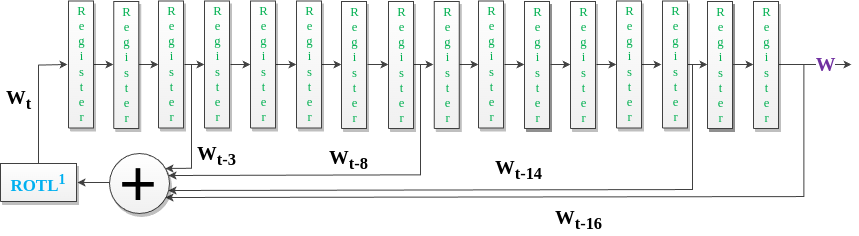
\includegraphics[width= 0.9\textwidth]{figure_5.18}\\
\caption{ SHA1 message schedule }
\label{fig:figure_5.18}
\end{figure}


The implementation of sha1\_core is depicted in Figure \ref{fig:figure_5.19}. Its inputs are the input block, the values $H_0^{(i-1)}, H_1^{(i-1)}, H_2^{(i-1)}, H_3^{(i-1)}, H_4^{(i-1)}$, and the clock ($clk$) and reset ($rst$) signals. The $H$ values are also needed as inputs because, as can be observed in the pseudocode in Algorithm \ref{alg:hmac_pre}, the new $H$ values are calculated using the previous ones. Thus, as will be explained in the sha1 unit description, there is an external feedback loop from the output of the sha1\_core into $H_0^{(i)}, H_1^{(i)}, H_2^{(i)}, H_3^{(i)}, H_4^{(i)}$. sha1 outputs the computed hash value and a signal hash\_rd which indicates that the processing of this block has finished.

% fig 5.19
\begin{figure}[H]
\centering
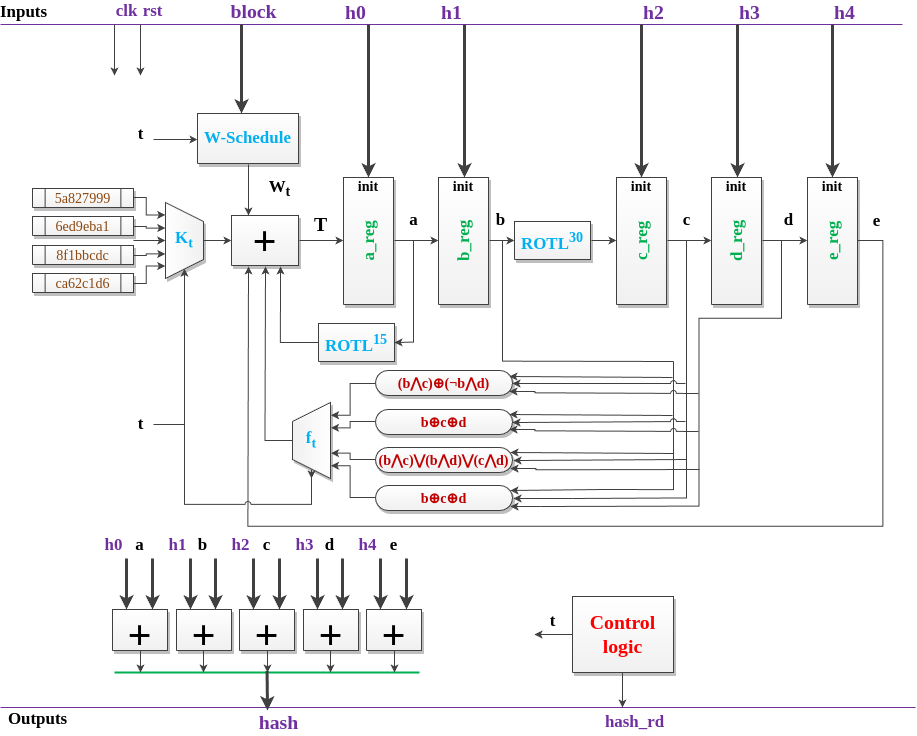
\includegraphics[width= 0.8\textwidth]{figure_5.19}\\
\caption{ sha1\_core module implementation }
\label{fig:figure_5.19}
\end{figure}


In Figure \ref{fig:figure_5.19}, the variable $t$ corresponds to the number of current iterations. The 5 registers connected in series (a\_reg to e\_reg) implement the assignments in line ~\ref{hmac:asign1}. The calculation of line ~\ref{hmac:T} is broken down to:

\begin{outline}
    \1 The calculation of $f_t$ (\ref{eq:f_t}) is performed through four segments of digital logic and a multiplexer among these four. The MUX selection is based on $t$
    \1 The signal $K_t$ (\ref{eq:K_t}) is assigned one of the four constant values depending on the value of $t$
    \1 The $W_t$ is computed by the W-Schedule unit
    \1 $ROTL5(a)$ is calculated, and all the above, along with $e$, are fed into an addition unit whose output is the value of $T$ 
    \1 the value of $T$ is stored into the $a\_reg$ in order to implement the final assignment $a = T$
\end{outline}

The output values (line ~\ref{hmac:asign2}) are computed using adders. The control logic includes a counter that is initialized to '0' with every rst and has a maximum value of '79', which keeps until a new rst signal is given. The value of $t$ corresponds to the value of this counter. Furthermore, the control logic raises the output signal hash\_rd when the counter reaches the value '79' to indicate that all iterations have been executed.

% fig 5.20
\begin{figure}[H]
\centering
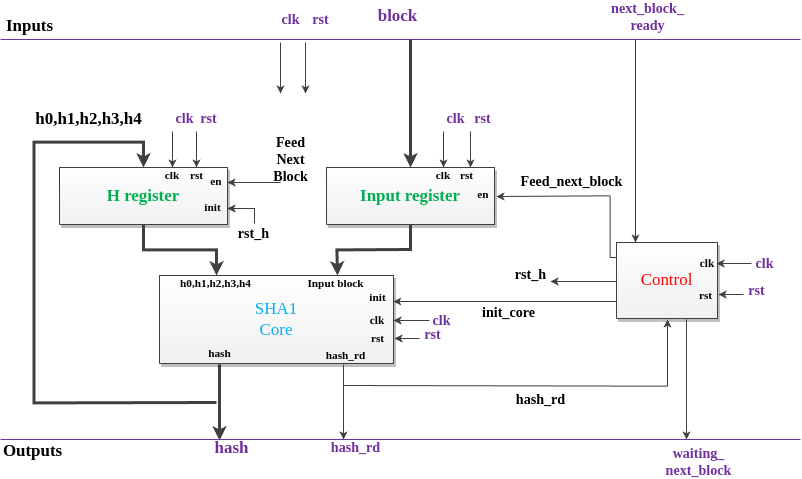
\includegraphics[width= 0.8\textwidth]{figure_5.20}\\
\caption{ sha1 module implementation}
\label{fig:figure_5.20}
\end{figure}

The sha1 unit takes as input the message's current block, the control signal next\_block\_ready which notifies the unit that a new block is available at its input, and the clock (clk) and reset (rst) signals. It outputs the result of the hash computation, the hash\_rd signal indicating the end of hash computation for the current block, and a waiting\_next\_block signal indicating that the unit is ready to accept a new block at its input. The block diagram of the implementation is shown in Figure \ref{fig:figure_5.20}.

The design consists of a sha1\_core, two registers, and a control unit. The input register serves as a buffer that holds the input block, allowing a new block to be placed at the unit's input without affecting the ongoing operation. The H register is used to feed back the values $H_0^{(i-1)}, H_1^{(i-1)}, H_2^{(i-1)}, H_3^{(i-1)},$ and $H_4^{(i-1)}$ for processing the next block, which implements the assignments in line ~\ref{hmac:assign3}.

% fig 5.21
\begin{figure}
\centering
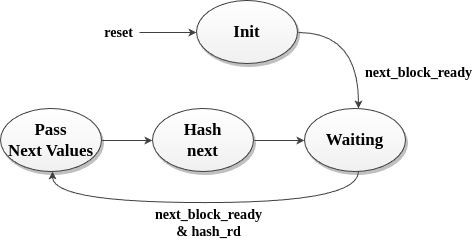
\includegraphics[width= 0.6\textwidth]{figure_5.21}\\
\caption{  sha1 control FSM }
\label{fig:figure_5.21}
\end{figure}

The operation of the control unit is described through the FSM diagram in Figure \ref{fig:figure_5.21}. For starting a hash computation of a new message, a reset signal needs to be issued that places us in the Init state. In this state, the H register is set to the initial values (line ~\ref{hmac:init_H}) and initializes the sha1\_core unit with the internal signal Init\_core. When entering the Init state, the waiting\_next\_block is issued.

After the first block is provided at the input the the next\_block\_ready signal is issued and that transitions the FSM to the Waiting state where the 80 iterations are executed for the first block. In this state, the control unit waits for the sha1\_core to finish processing, which is indicated by the hash\_rd signal, and for the next\_block\_ready signal to be given (after placing the next block at the input). When both conditions are met, the FSM transitions to the Pass Next Values state, where a pulse of the internal signal feed\_next\_block is issued so that the new values of $H$ and the next block are provided to the sha1\_core input. After one clock cycle, the FSM transitions to the Hash next state, where the sha1\_core has taken the new values at its inputs, and then automatically transitions to the Waiting state where the 80 iterations are executed for the current block. This process repeats until all blocks are provided.

The last unit implemented is the hmac\_sha1\_96, whose block diagram is shown in Figure \ref{fig:figure_5.22}. At its input, it receives the key, one message block msg\_block, the control signals next\_block and msg\_done, and the clock and reset signals. The next\_block signal is used to indicate that the next block is at the msg\_block input, while the msg\_done signal indicates that we are providing the last block of the message. Its outputs include the computed MAC and the signals waiting\_nxt and ready. The waiting\_nxt signal indicates that the unit is ready to accept a new block at its input, and ready indicates the end of the MAC computation.

% fig 5.22
\begin{figure}
\centering
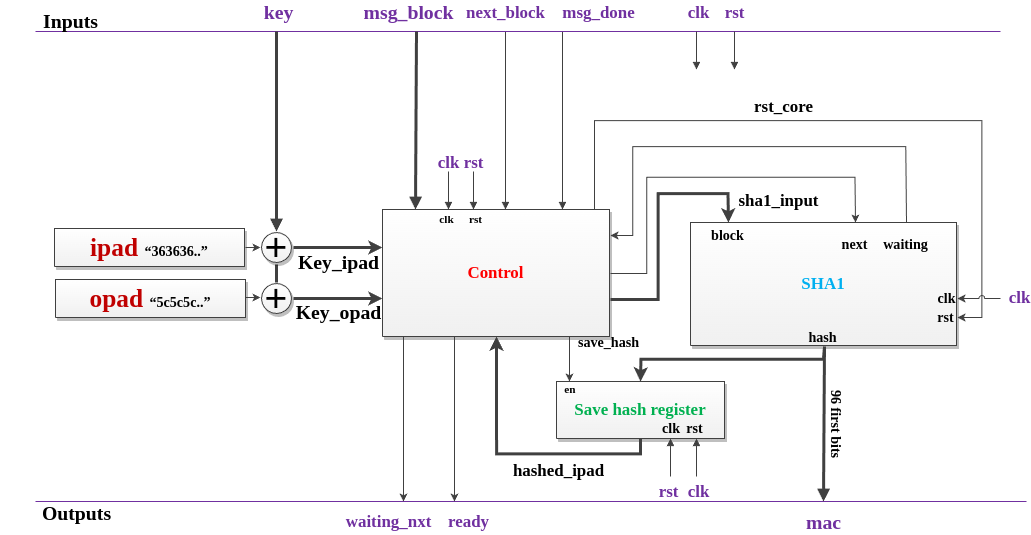
\includegraphics[width= 0.8\textwidth]{figure_5.22}\\
\caption{ hmac\_sha1\_96 module implementation}
\label{fig:figure_5.22}
\end{figure}

The unit consists includes the constants $ipad$ and $opad$, two bitwise XOR operations between these constants and the key, a sha1 unit, a register to store the intermediate calculation of $H((K_0 \oplus ipad) || text)$, and a control unit.

The control unit is responsible for routing the appropriate value to the input of the sha1 unit. This is depicted in Figure \ref{fig:figure_5.22} with the values of $K_0\oplus ipad$, $K_0\oplus opad$, hashed\_ipad, and msg\_block being provided to the control unit. The control unit's FSM is presented in Figure \ref{fig:figure_5.23}.

For each new calculation of HMAC-SHA1-96, the unit is first initialized with a reset signal leading the FSM to the Start state. In this state, the sha1 unit is initialized through a pulse issued on the internal signal rst\_core, while the signal waiting\_nxt is kept active indicating that the unit is ready to accept the first block. Once the first block is provided and the next\_block signal is issued, the FSM transitions to the $Hash(key\oplus ipad)$ state. There the first block of the message $(K_0\oplus ipad) || text$, $(K_0\oplus ipad)$, is routed to the sha1 unit. Once the calculation is completed, the waiting\_next\_block signal of the sha1 unit is issued, and the FSM transitions to the Hash \nth{1} block state, where the first block of the message is given to the sha1 unit. After this calculation finishes, the FSM enters the loop of states Wait Next Block and Hash Next Block. In the Wait Next Block state, the unit waits for the next block, and once provided, it moves to the Hash Next Block state to perform the next calculation on the newly provided block. This process continues until the msg\_done signal is issued, indicating that all blocks of the message have been provided, and therefore, the output of the sha1 unit has the quantity $H((K_0\oplus ipad) || text)$.

When the msg\_done signal is issued, the FSM transitions to the Save Hash state, where the value $H((K_\oplus ipad) || text)$ is stored in the Save Hash Register using the save\_hash signal. In the next clock cycle, the FSM automatically moves to the Reset Core state, where the sha1 unit gets prepared for a new calculation. When the sha1 unit is ready, the calculation $H[(K_0\oplus opad) || H((K_0\oplus ipad) || text)]$ starts. In the $Hash(key\oplus opad)$ state, the block $(K_0\oplus opad)$ is given to the sha1 unit. Once the calculation is finished (i.e., when waiting\_next\_block='1'), the \nth{2} block of the message is provided, $H((K_0\oplus ipad) || text)$. At the end of this calculation, the final MAC value is available at the output of the sha1 unit. The system moves to the Done state, where it issues the ready signal to indicate that the MAC is ready. The first 96 bits of the sha1 result are present at the output of the hmac\_sha1\_96.

% fig 5.23
\begin{figure}
\centering
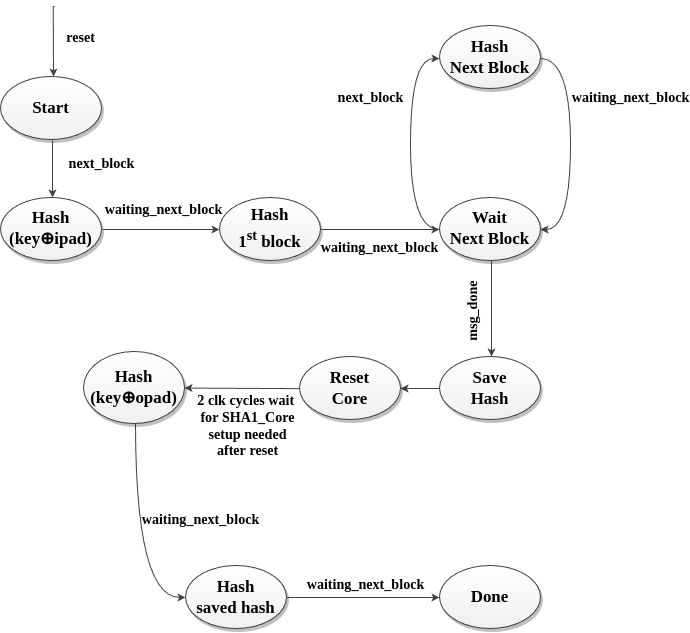
\includegraphics[width= 0.8\textwidth]{figure_5.23}\\
\caption{  hmac\_sha1\_96 control FSM }
\label{fig:figure_5.23}
\end{figure}

\section{Hardware-side Interface}
The interfaces of the two peripheral systems, CBC-AES-128 and HMAC-SHA1-96, are not fully suitable for direct connection to the processor bus. Their inputs and outputs need to be represented with registers corresponding to memory locations of the processor's address space (memory-mapped IO).

Xilinx's toolset offers a procedure for creating and connecting custom-designed peripheral systems. This type of peripheral is referred to by Xilinx as a custom IP core. Through this process, these peripherals and their interfaces are defined. In the case of CBC-AES-128, the interface consists of 17 32-bit registers, of which 4 are used for the input block, 4 for the output block, 4 for the key, 4 for the IV, and the last one serves as a command/status register. The last register, when read by the processor, provides peripheral notification signals, while when written, it sets the peripheral's command signals. It is worth noting that the 4 registers of the output block could overlap with some of the input registers since the former are used only for writing and the latter only for reading. A choice to separate them is made solely to keep the design clear. For HMAC-SHA1-96, there are a total of 36 32-bit registers. 16 are dedicated to the input block, 16 to the key, 3 to its output (a 96-bit MAC), and one is the command/status register. As several bits in the command/status registers remain unused, some signals are exposed through them to assist with the debugging of the peripherals.
